\documentclass[tikz,border=8pt]{standalone}

\usepackage[T1]{fontenc}
\usepackage{lmodern}
\usetikzlibrary{arrows.meta,backgrounds,calc,fit,positioning}

\definecolor{perception}{HTML}{DCEBFF}
\definecolor{decision}{HTML}{E4F4E8}
\definecolor{critic}{HTML}{FFF0D6}
\definecolor{runtime}{HTML}{F1E7FF}
\definecolor{linegray}{HTML}{4A5568}
\definecolor{textgray}{HTML}{1A202C}

\tikzset{
  font=\sffamily,
  every node/.style={text=textgray},
  block/.style={
    draw=linegray,
    rounded corners=2pt,
    very thick,
    align=center,
    minimum height=12mm,
    text width=34mm,
    inner sep=4pt
  },
  smallblock/.style={
    block,
    minimum height=9mm,
    text width=29mm,
    font=\sffamily\footnotesize
  },
  wideblock/.style={
    block,
    text width=43mm
  },
  note/.style={
    draw=linegray,
    rounded corners=2pt,
    align=center,
    text width=35mm,
    inner sep=4pt,
    font=\sffamily\scriptsize
  },
  group/.style={
    draw=linegray,
    rounded corners=3pt,
    dashed,
    inner sep=7pt
  },
  flow/.style={-Latex, very thick, draw=linegray},
  skip/.style={-Latex, very thick, draw=linegray, dashed},
  thinflow/.style={-Latex, thick, draw=linegray},
  label/.style={font=\sffamily\scriptsize, align=center}
}

\begin{document}
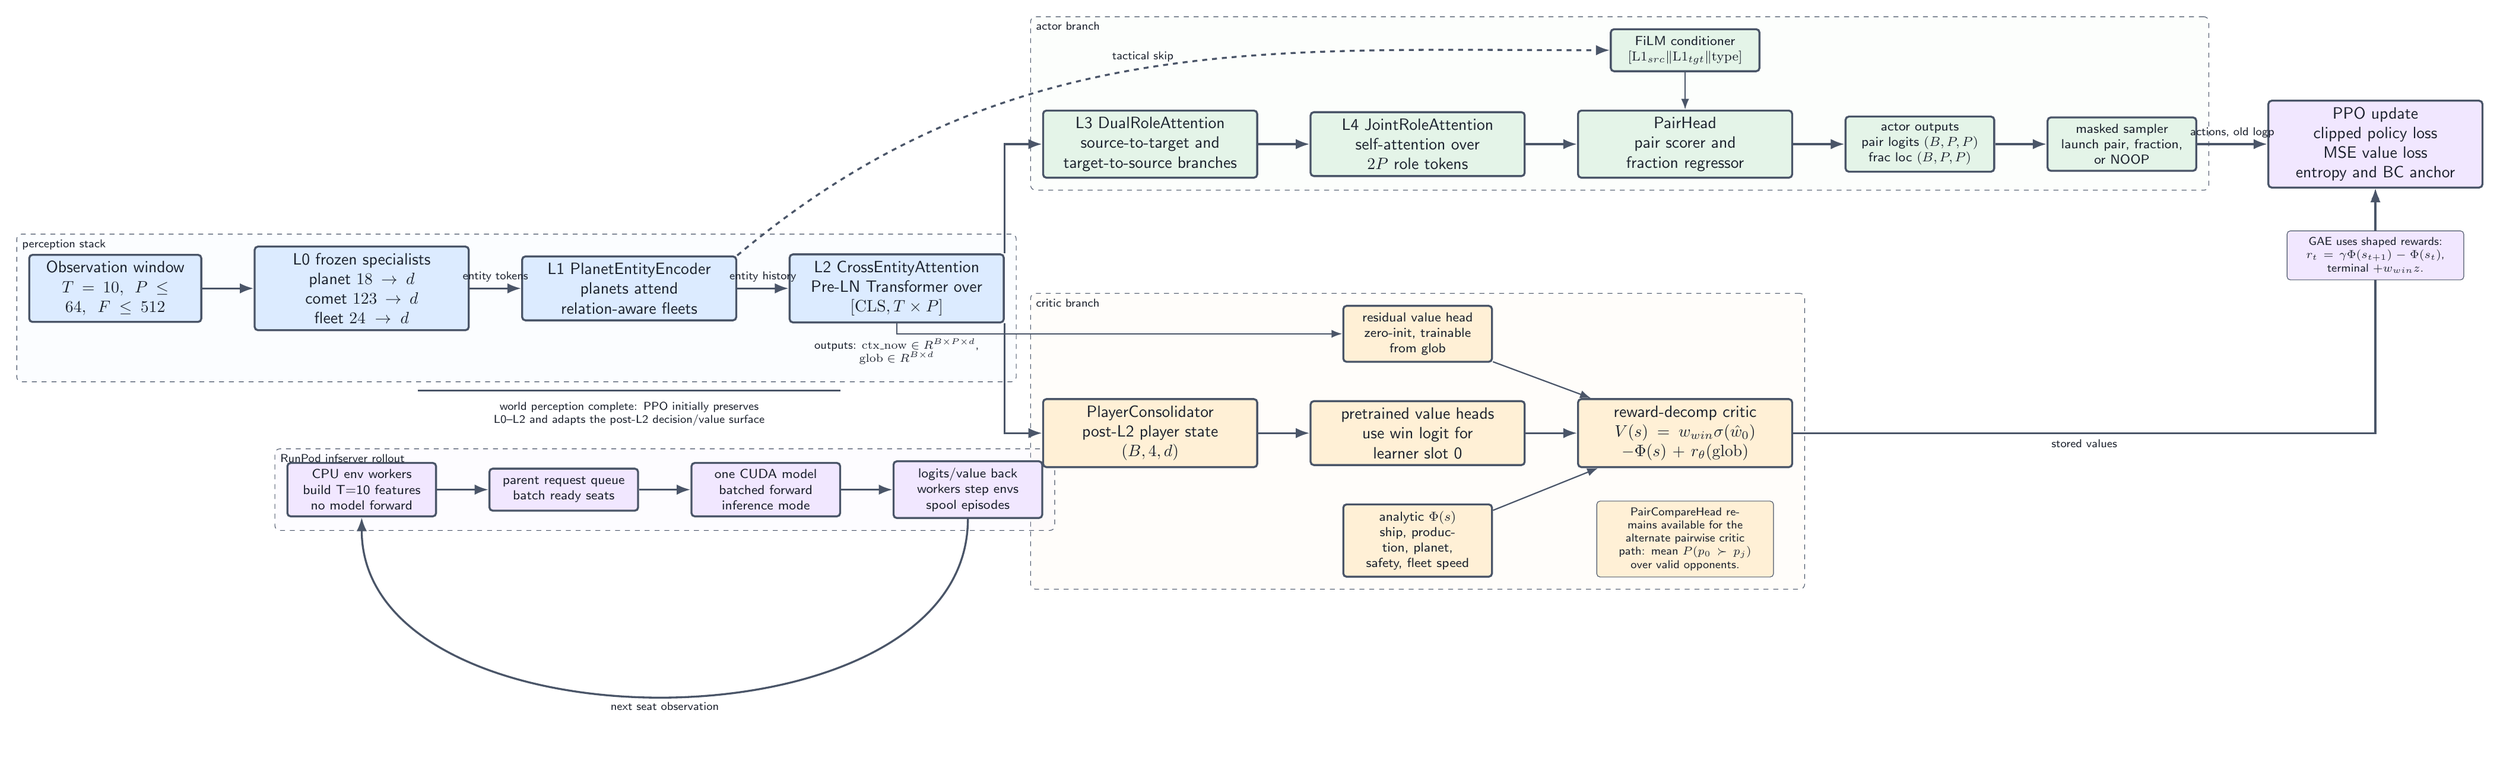
\begin{tikzpicture}[node distance=9mm and 11mm]

% --------------------------------------------------------------------------
% Main model path
% --------------------------------------------------------------------------
\node[block, fill=perception] (obs) {
  Observation window\\
  $T=10,\; P\le64,\; F\le512$
};

\node[wideblock, fill=perception, right=of obs] (l0) {
  L0 frozen specialists\\
  planet $18\!\to\!d$\\
  comet $123\!\to\!d$\\
  fleet $24\!\to\!d$
};

\node[wideblock, fill=perception, right=of l0] (l1) {
  L1 PlanetEntityEncoder\\
  planets attend relation-aware fleets
};

\node[wideblock, fill=perception, right=of l1] (l2) {
  L2 CrossEntityAttention\\
  Pre-LN Transformer over\\
  $[\mathrm{CLS}, T\!\times\!P]$
};

\node[label, below=2mm of l2] (l2out) {
  outputs: $\mathrm{ctx\_now}\in\mathbb{R}^{B\times P\times d}$,\\
  $\mathrm{glob}\in\mathbb{R}^{B\times d}$
};

\draw[flow] (obs) -- (l0);
\draw[flow] (l0) -- node[label, above] {entity tokens} (l1);
\draw[flow] (l1) -- node[label, above] {entity history} (l2);

\node[label, below=16mm of l1, text width=80mm] (boundary) {
  world perception complete: PPO initially preserves L0--L2 and adapts the post-L2 decision/value surface
};
\draw[very thick, linegray] ($(boundary.west)+(-4mm,5mm)$) -- ($(boundary.east)+(4mm,5mm)$);

% --------------------------------------------------------------------------
% Actor branch
% --------------------------------------------------------------------------
\node[wideblock, fill=decision, above right=16mm and 8mm of l2] (l3) {
  L3 DualRoleAttention\\
  source-to-target and\\
  target-to-source branches
};

\node[wideblock, fill=decision, right=of l3] (l4) {
  L4 JointRoleAttention\\
  self-attention over\\
  $2P$ role tokens
};

\node[wideblock, fill=decision, right=of l4] (pairhead) {
  PairHead\\
  pair scorer and\\
  fraction regressor
};

\node[smallblock, fill=decision, above=8mm of pairhead] (film) {
  FiLM conditioner\\
  $[\mathrm{L1}_{src}\Vert\mathrm{L1}_{tgt}\Vert\mathrm{type}]$
};

\node[smallblock, fill=decision, right=of pairhead] (actorout) {
  actor outputs\\
  pair logits $(B,P,P)$\\
  frac loc $(B,P,P)$
};

\node[smallblock, fill=decision, right=of actorout] (sampler) {
  masked sampler\\
  launch pair, fraction,\\
  or NOOP
};

\draw[flow] (l2.north east) |- (l3.west);
\draw[flow] (l3) -- (l4);
\draw[flow] (l4) -- (pairhead);
\draw[flow] (pairhead) -- (actorout);
\draw[flow] (actorout) -- (sampler);
\draw[skip] (l1.north east) to[out=40,in=180] node[label, above] {tactical skip} (film.west);
\draw[thinflow] (film) -- (pairhead);

% --------------------------------------------------------------------------
% Critic branch
% --------------------------------------------------------------------------
\node[wideblock, fill=critic, below right=16mm and 8mm of l2] (consolidator) {
  PlayerConsolidator\\
  post-L2 player state\\
  $(B,4,d)$
};

\node[wideblock, fill=critic, right=of consolidator] (winhead) {
  pretrained value heads\\
  use win logit for\\
  learner slot 0
};

\node[smallblock, fill=critic, above=8mm of winhead] (resid) {
  residual value head\\
  zero-init, trainable\\
  from glob
};

\node[smallblock, fill=critic, below=8mm of winhead] (phi) {
  analytic $\Phi(s)$\\
  ship, production, planet,\\
  safety, fleet speed
};

\node[wideblock, fill=critic, right=of winhead] (value) {
  reward-decomp critic\\
  $V(s)=w_{win}\sigma(\hat w_0)$\\
  $-\Phi(s)+r_\theta(\mathrm{glob})$
};

\node[note, fill=critic, below=7mm of value] (altcritic) {
  PairCompareHead remains available for the alternate pairwise critic path:
  mean $P(p_0 \succ p_j)$ over valid opponents.
};

\draw[flow] (l2.south east) |- (consolidator.west);
\draw[flow] (consolidator) -- (winhead);
\draw[thinflow] (l2) |- (resid.west);
\draw[thinflow] (resid) -- (value);
\draw[thinflow] (phi) -- (value);
\draw[flow] (winhead) -- (value);

% --------------------------------------------------------------------------
% PPO objective
% --------------------------------------------------------------------------
\node[wideblock, fill=runtime, right=15mm of sampler] (ppo) {
  PPO update\\
  clipped policy loss\\
  MSE value loss\\
  entropy and BC anchor
};
\draw[flow] (sampler) -- node[label, above] {actions, old logp} (ppo);
\draw[flow] (value.east) -| node[label, near start, below] {stored values} (ppo.south);

\node[note, fill=runtime, below=9mm of ppo] (gae) {
  GAE uses shaped rewards:\\
  $r_t=\gamma\Phi(s_{t+1})-\Phi(s_t)$, terminal $+w_{win}z$.
};
\draw[thinflow] (gae) -- (ppo);

% --------------------------------------------------------------------------
% Runtime infserver side panel
% --------------------------------------------------------------------------
\node[smallblock, fill=runtime, below=28mm of l0] (workers) {
  CPU env workers\\
  build T=10 features\\
  no model forward
};

\node[smallblock, fill=runtime, right=of workers] (queue) {
  parent request queue\\
  batch ready seats
};

\node[smallblock, fill=runtime, right=of queue] (gpu) {
  one CUDA model\\
  batched forward\\
  inference mode
};

\node[smallblock, fill=runtime, right=of gpu] (reply) {
  logits/value back\\
  workers step envs\\
  spool episodes
};

\draw[flow] (workers) -- (queue);
\draw[flow] (queue) -- (gpu);
\draw[flow] (gpu) -- (reply);
\draw[flow] (reply.south) to[out=-90,in=-90,looseness=1.0] node[label, below] {next seat observation} (workers.south);

% --------------------------------------------------------------------------
% Group boxes
% --------------------------------------------------------------------------
\begin{scope}[on background layer]
  \node[group, fill=perception, fill opacity=0.12,
        fit=(obs) (l0) (l1) (l2) (l2out)] (perceptionGroup) {};
  \node[group, fill=decision, fill opacity=0.12,
        fit=(l3) (l4) (pairhead) (film) (actorout) (sampler)] (actorGroup) {};
  \node[group, fill=critic, fill opacity=0.12,
        fit=(consolidator) (winhead) (resid) (phi) (value) (altcritic)] (criticGroup) {};
  \node[group, fill=runtime, fill opacity=0.12,
        fit=(workers) (queue) (gpu) (reply)] (runtimeGroup) {};
\end{scope}

\node[label, anchor=north west] at (perceptionGroup.north west) {perception stack};
\node[label, anchor=north west] at (actorGroup.north west) {actor branch};
\node[label, anchor=north west] at (criticGroup.north west) {critic branch};
\node[label, anchor=north west] at (runtimeGroup.north west) {RunPod infserver rollout};

\end{tikzpicture}
\end{document}
